\documentclass{bioinfo}
\copyrightyear{2015} \pubyear{2015}

\access{Advance Access Publication Date: Day Month Year}
\appnotes{Manuscript Category}

\usepackage{adjustbox}
\usepackage{multirow}
\usepackage{graphicx}
\graphicspath{{../figures/}}
\usepackage{xr}
\externaldocument{bigsnpr-review-supp}


\begin{document}
\firstpage{1}

\subtitle{Subject Section}

\title[R packages for analyzing genome-wide data]{Efficient management and analysis of large-scale genome-wide data with two R packages: bigstatsr and bigsnpr}
\author[Sample \textit{et~al}.]{Florian Priv\'e\,$^{\text{\sfb 1,}*}$, Hugues Aschard\,$^{\text{\sfb 2,\sfb 3}}$ and Michael G.B. Blum\,$^{\text{\sfb 1,}*}$}
\address{$^{\text{\sf 1}}$Universit\'e Grenoble Alpes, CNRS, Laboratoire TIMC-IMAG, UMR 5525, France, \\
$^{\text{\sf 2}}$Centre de Bioinformatique, Biostatistique et Biologie Int\'egrative (C3BI), Institut Pasteur, Paris, France and \\
$^{\text{\sf 3}}$Department of Epidemiology, Harvard T.H. Chan School of Public Health, Boston, Massachusetts, USA.}

\corresp{$^\ast$To whom correspondence should be addressed.}

\history{Received on XXXXX; revised on XXXXX; accepted on XXXXX}

\editor{Associate Editor: XXXXXXX}

\abstract{\textbf{Motivation:} Genome-wide datasets produced for association studies have dramatically increased in size over the past few years, with modern datasets commonly including millions of variants measured in dozens of thousands of individuals. This increase in data size is a major challenge severely slowing down genomic analyses. Specialized software for every part of the analysis pipeline have been developed to handle large genomic data. However, combining all these software into a single data analysis pipeline might be technically difficult. \\
\textbf{Results:} Here we present two R packages, bigstatsr and bigsnpr, allowing for management and analysis of large scale genomic data to be performed within a single comprehensive framework. To address large data size, the packages use memory-mapping for accessing data matrices stored on disk instead of in RAM. To perform data pre-processing and data analysis, the packages integrate most of the tools that are commonly used, either through transparent system calls to existing software, or through updated or improved implementation of existing methods. In particular, the packages implement a fast derivation of Principal Component Analysis, functions to remove SNPs in Linkage Disequilibrium, and algorithms to learn Polygenic Risk Scores on millions of SNPs. We illustrate applications of the two R packages by analysing a case-control genomic dataset for the celiac disease, performing an association study and computing Polygenic Risk Scores. Finally, we demonstrate the scalability of the R packages by analyzing a simulated genome-wide dataset including 500,000 individuals and 1 million markers on a single desktop computer. \\
\textbf{Availability:} \href{https://privefl.github.io/bigstatsr/}{https://privefl.github.io/bigstatsr/} \& \href{https://privefl.github.io/bigsnpr/}{https://privefl.github.io/bigsnpr/}\\
\textbf{Contact:} \href{florian.prive@univ-grenoble-alpes.fr}{florian.prive@univ-grenoble-alpes.fr} \& \href{michael.blum@univ-grenoble-alpes.fr}{michael.blum@univ-grenoble-alpes.fr}\\
\textbf{Supplementary information:} Supplementary data are available at \textit{Bioinformatics}
online.}

\maketitle

\section{Introduction}

Genome-wide datasets produced for association studies have dramatically increased in size over the past years. A range of software and data formats have been developed to perform essential pre-processing steps and data analysis, often optimizing each of these steps within a dedicated implementation. This diverse and extremely rich software environment has been of tremendous benefit for the genetic community. However, it has two limitations: analysis pipelines are becoming very complex and researchers have limited access to diverse analysis tools due to growing data sizes.

Consider first the basic tools necessary to perform a standard genome-wide analysis. Conversions between standard file formats has become a field by itself with several tools such as VCFtools, BCFtools and PLINK, available either independently or incorporated within large framework \cite[]{Danecek2011,Li2011,Purcell2007}. Similarly, quality control software for genome-wide analysis have been developed such as PLINK and the Bioconductor package GWASTools \cite[]{Gogarten2012}.
There are also several software for the computation of principal components (PCs) of genotypes, commonly performed to account for population stratification in association studies, including EIGENSOFT (SmartPCA and FastPCA) and FlashPCA \cite[]{Abraham2014a,Abraham2016a,Galinsky2016,Price2006}.
Then, implementation of GWAS analyses also depends on the data format and model analyzed. For example, the software ProbABEL \cite[]{Aulchenko2010} or SNPTEST \cite[]{Marchini2010} can handle dosage data, while PLINK version 1.9 is limited to best guess genotypes because of its input file format. Note that PLINK 2.0 will completely handle this type of data, but is still in the alpha stage of development. 
Finally, there exists a range of tools for Polygenic Risk Scores (PRSs) such as LDpred \cite[]{Vilhjalmsson2015} and PRSice \cite[]{Euesden2015}, which provide prediction for quantitative traits or disease risks based on multiple genetic variants. As a result, one has to make extensive bash/perl/R/python scripts to link these software together and convert between multiple file formats, involving many file manipulations and conversions. Overall, this might be a barrier to data exploration. 
%Overall, this means that researchers are usually restricted on how they can manipulate and analyse the data they have access to.

Secondly, increasing size of genetic datasets is the source of major computational challenges and many analytical tools would be restricted by the amount of memory (RAM) available on computers. This is particularly a burden for commonly used analysis languages such as R, Python and Perl. Solving the memory issues for these languages would give access to a broad range of tools for data analysis that have been already implemented. Hopefully, strategies have been developed to avoid loading large datasets in RAM. For storing and accessing matrices, memory-mapping is very attractive because it is seamless and usually much faster to use than direct read or write operations. Storing large matrices on disk and accessing them via memory-mapping has been available for several years in R through ``big.matrix'' objects implemented in the R package bigmemory \cite[]{Kane2013}.

%\enlargethispage{12pt}

\section{Approach}

{\color{red}
In order to perform analyses of large-scale genomic data in R, we developed two R packages, bigstatsr and bigsnpr, that provide a wide-range of building blocks which are parts of standard analyses. 
For instance, one might like using R because R makes it easy to tie together (existing or new) functions to be used as part of large, interactive and reproducible analyses.
We provide a similar format as filebacked ``big.matrix'' objects that we called ``Filebacked Big Matrices (FBMs)''. Thanks to this matrix-like format, algorithms in R/C++ can be developed or adapted for large genotype data. This data format is a particularly good trade-off between easiness of use and computation efficiency, making our code both simple and fast.
}
Package bigstatsr implements many statistical tools for several types of FBMs (unsigned char, unsigned short, integer and double). This includes implementation of multivariate sparse linear models, Principal Component Analysis, matrix operations, and numerical summaries. The statistical tools developed in bigstatsr can be used for other types of data as long as they can be represented as matrices. Package bigsnpr depends on bigstatsr, using a special type of FBM object to store the genotypes, called ``FBM.code256''. Package bigsnpr implements algorithms which are specific to the analysis of SNP arrays, such as calls to external software for processing steps, I/O (Input/Output) operations from binary PLINK files, and data analysis operations on SNP data (thinning, testing, predicting, plotting). 
We use both a real case-control genomic dataset for Celiac disease and large-scale simulated data to illustrate application of the two R packages, including association study and computation of Polygenic Risk Scores. We also compare results from the two R packages with those obtained when using PLINK and EIGENSOFT, and report execution times along with the code to perform major computational tasks.


\begin{methods}
\section{Methods}

\subsection{Memory-mapped files}

The two R packages do not use standard read operations on a file nor load the genotype matrix entirely in memory. They use an hybrid solution: memory-mapping. Memory-mapping is used to access data, possibly stored on disk, as if it were in memory. This solution is made available within R through the BH package, providing access to Boost C++ Header Files\footnote{http://www.boost.org/}.

We are aware of the software library SNPFile that uses memory-mapped files to store and efficiently access genotype data, coded in C++ \cite[]{Nielsen2008} and of the R package BEDMatrix\footnote{https://github.com/QuantGen/BEDMatrix} which provides memory-mapping directly for binary PLINK files. With the two packages we developed, we made this solution available in R and in C++ via package Rcpp \cite[]{Eddelbuettel2011}. The major advantage of manipulating genotype data within R, almost as it were a standard matrix in memory, is the possibility of using most of the other tools that have been developed in R \cite[]{R2017}. For example, we provide sparse multivariate linear models and an efficient algorithm for Principal Component Analysis (PCA) based on adaptations from R packages biglasso and RSpectra \cite[]{RSpectra2016,Zeng2017}.

Memory-mapping provides transparent and faster access than standard read/write operations. 
When an element is needed, a small chunk of the genotype matrix, containing this element, is accessed in memory. 
When the system needs more memory, some chunks of the matrix are freed from the memory in order to make space for others. 
All this is managed by the Operating System so that it is seamless and efficient. 
It means that if the same chunks of data are used repeatedly, it will be very fast the second time they are accessed, the third time and so on. 
Of course, if the memory size of the computer is larger than the size of the dataset, the file could fit entirely in memory and every second access would be fast. 


\subsection{Data management, preprocessing and imputation} \label{sec:preprocess}

{\color{red}
We developed a special FBM object, called ``FBM.code256'', that can be used to seamlessly store up to 256 arbitrary different values, while having a relatively efficient storage. Indeed, each element is stored on one byte which requires 8 times less disk storage than double-precision numbers but 4 times more space than the binary PLINK format ``.bed'' which can store only genotype calls. With these 256 values, the matrix can store genotype calls and missing values (4 values), best guess genotypes (3 values) and genotype dosages (likelihoods) rounded to two decimal places (201 values). So, we use a single data format that can store both genotype calls and dosages.

For preprocessing steps, we think the user should use PLINK, which is an invaluable tool for this. For the sake of reproducibility, one could use PLINK directly from R via systems calls. For the sake of simplicity, we provide wrappers as R functions that use system calls to PLINK for the conversion and quality control steps with as input a variety of formats (e.g. vcf, bed/bim/fam, ped/map) and bed/bim/fam files as output (Figure~\ref{fig:qc}).
Package bigsnpr provides fast conversions between bed/bim/fam PLINK files and the ``bigSNP'' object, which contains the genotype Filebacked Big Matrix (FBM.code256), a data frame with information on samples and another data frame with information on SNPs. We also provide another function which could be used to read from tabular-like text files in order to create a genotype in the format ``FBM''. Finally, we provide two methods for reading-in dosages as proof of concept and will provide a more final solution when we get access to the UK Biobank dataset ([SUPPMAT]).

Most modern SNP chips provide genotype data with large call-rates. For example, the Celiac data we use in this paper present only a proportion of 0.0004 of missing values for the genotyped SNPs after quality control. Yet, most of the functions in bigstatsr and bigsnpr do not handle missing values.
So, we provide two functions for imputing missing values of genotyped SNPs. Note that we do not impute completely missing SNPs which would require the use of reference panels and could be performed via e.g. imputation servers for human data \cite[]{mccarthy2016reference}. The first function is a wrapper to PLINK and Beagle \cite[]{Browning2009} which takes bed files as input and return bed files without missing values, and should therefore be used before reading the data in R (Figure~\ref{fig:impute}). Beagle uses phasing before imputing, which could take several weeks even when there are only a tiny amount of missing values to be imputed. The second function is a new algorithm we developed in order to have a fast imputation method without losing much of imputation accuracy. We also provide an accurate estimation of the number of errors of imputation by SNP for post quality control.
This algorithm is based on Machine Learning approaches for genetic imputation \cite[]{Wang2012} and does not use phasing, thus allowing for a dramatic decrease in computation time. It only relies on some local XGBoost models. XGBoost is an optimized distributed gradient boosting library that can be used in R and provides some of the best results in machine learning competitions \cite[]{Chen2016}.
XGBoost builds decision trees that can detect nonlinear interactions, partially reconstructing phase, making it well suited for imputing genotype matrices. 
Our algorithm is the following: for each SNP, we divide the individuals in the ones which have a missing genotype (test set) and the ones which have a non-missing genotype for this particular SNP. Those latter individuals are further separated in a training set and a validation set (e.g. 80\% training and 20\% validation). The training set is used to build the XGBoost model for predicting missing data. The prediction model is then evaluated on the validation set for which we know the true genotype values, which gives an unbiased estimator of the number of genotypes that have been wrongly imputed for that particular SNP. The prediction model is also projected on the test set (missing values) in order to impute them.
}



\subsection{Population structure and SNP thinning based on Linkage Disequilibrium} 



For computing Principal Components (PCs) of a large-scale genotype matrix, we provide several functions related to SNP thinning and two functions, for computing a partial Singular Value Decomposition (SVD), one based on eigenvalue decomposition, big\_SVD, and the other on randomized projections, big\_randomSVD (Figure~\ref{fig:svd}). While the function based on eigenvalue decomposition is at least quadratic in the smallest dimension, the function based on randomized projections runs in linear time in all dimensions \cite[]{Lehoucq1996}. Package bigstatsr use the same PCA algorithm as FlashPCA2 called Implicitly Restarted Arnoldi Method (IRAM), which is implemented in R package RSpectra. The main difference between the two implementations is that FlashPCA2 computes vector-matrix multiplications with the genotype matrix based on the binary PLINK file whereas bigstatsr computes these multiplications based on the FBM format, which enables parallel computations and easier subsetting. 

\begin{figure}[!tpb]
\centerline{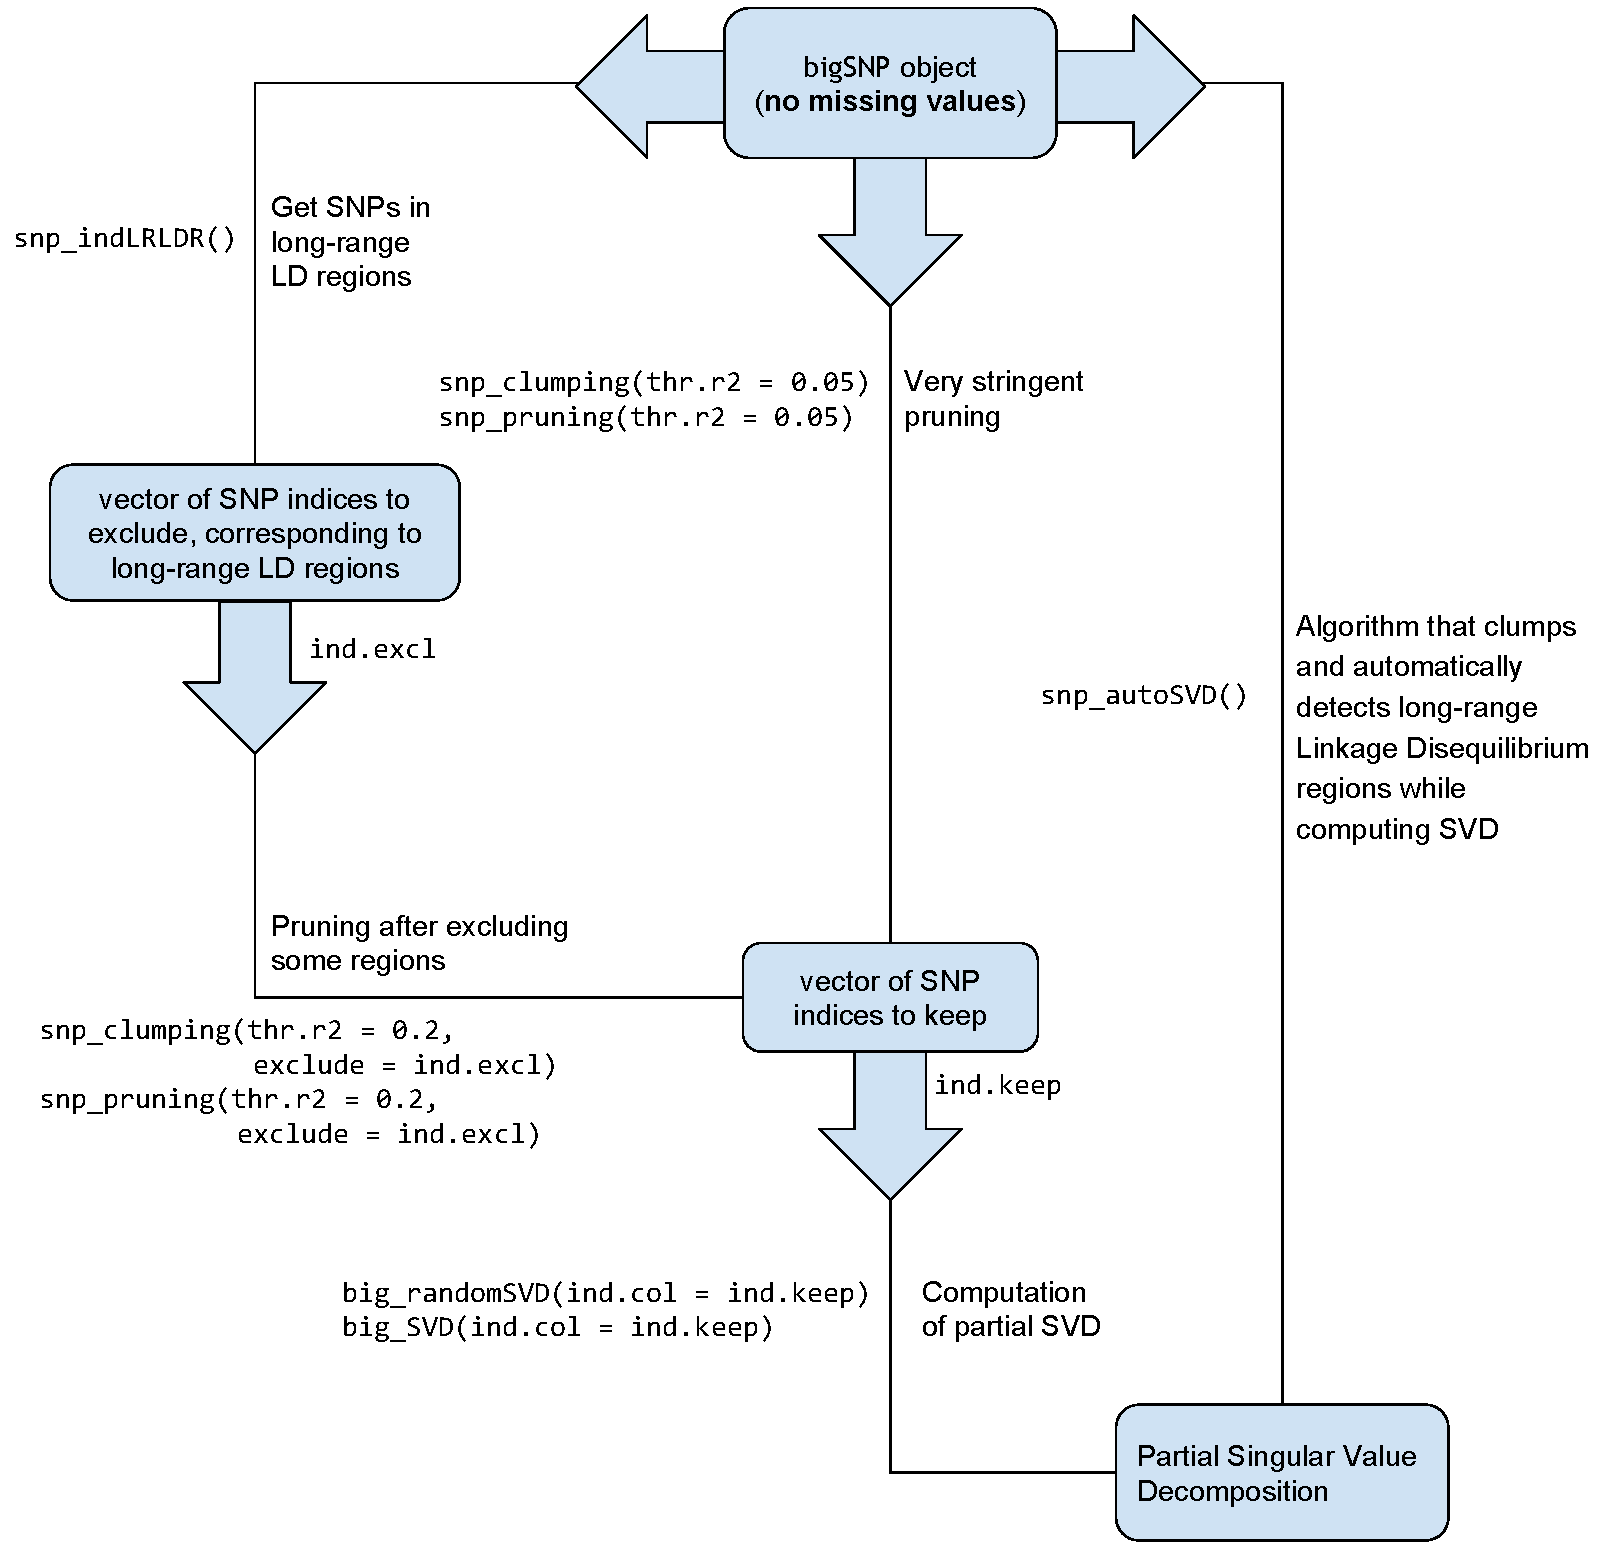
\includegraphics[width=235pt]{svd.pdf}}
\caption{Functions available in packages bigstatsr and bigsnpr for the computation of a partial Singular Value Decomposition of a genotype array, with 3 different methods for thinning SNPs.}\label{fig:svd}
\end{figure}
 
SNP thinning improves ascertainment of population structure with PCA \cite[]{Abdellaoui2013}. There are at least 3 different approaches to thin SNPs based on Linkage Disequilibrium, two of them named pruning and clumping, address SNPs in LD close to each others because of recombination events, while the third one address long-range regions with a complex LD pattern due to other biological events such as inversions \cite[]{Price2008}. 
First, pruning, the most naive approach, is an algorithm that sequentially scan the genome for nearby SNPs in LD, performing pairwise thinning based on a given threshold of correlation.
A variant of pruning is clumping. 
{\color{red}
Clumping is useful if a statistic is available to sort the SNPs by importance. Clumping is usually used to post-process results of a GWAS in order to keep only the most significant SNP per region of the genome. For PCA, the thinning procedure should remain unsupervised (one must not use any phenotype) and we therefore propose to use the minor allele frequency (MAF) as the statistic of importance. Note that this choice does not come out of nowhere because in the pruning algorithm of PLINK, when two nearby SNPs are correlated, only the one with the higher MAF is kept. Yet, in some worst-case scenario, the pruning algorithm can leave regions of the genome without any representative SNP at all so we advise to always use clumping instead of pruning, using the MAF as the statistic of importance, which is the default in function snp\_clumping ([SUPMAT]).
}

As mentioned above, the third approach that is generally combined with pruning or clumping consists of removing SNPs in long-range LD regions \cite[]{Price2008}. Long-range LD regions for the human genome are available as an online table that our packages can use to discard SNPs in long-range LD regions while computing PCs\footnote{https://goo.gl/8TngVE}. 
However, the pattern of LD might be population specific, so we developed an algorithm that automatically detects these regions and removes them. This algorithm consists in the following steps: first, PCA is performed using a subset of SNP remaining after clumping, then outliers SNPs are detected using Mahalanobis distance as implemented in the R package pcadapt \cite[]{Luu2017}. Finally, the algorithm considers that consecutive outlier SNPs are in long-range LD regions. Indeed, a long-range LD region would cause SNPs in this region to have strong consecutive weights (loadings) in the PCA. This algorithm is implemented in function snp\_autoSVD and will be referred by this name in the rest of the paper.


\subsection{Association tests and Polygenic Risk Scores}

Any test statistic that is based on counts could be easily implemented because we provide fast counting summaries. Among these tests, the Armitage trend test and the MAX3 test statistic are already provided for binary outcome \cite[]{Zheng2012}. 
We also implement statistical tests based on linear and logistic regressions. For the linear regression, for each SNP $j$, a t-test is performed on $\beta^{(j)}$ where
\begin{multline}
  \hat{y} = \alpha^{(j)} + \beta^{(j)} SNP^{(j)} + \gamma_1^{(j)} PC_1 + \cdots + \gamma_K^{(j)} PC_K \\ + \delta_1^{(j)} COV_1 + \cdots + \delta_K^{(j)} COV_L,
\end{multline}
and $K$ is the number of principal components and $L$ is the number of other covariates (such as the age and gender). Similarly, for the logistic regression, for each SNP $j$, a Z-test is performed on $\beta^{(j)}$ where
\begin{multline}
  \log{\frac{\hat{p}}{1-\hat{p}}} = \alpha^{(j)} + \beta^{(j)} SNP^{(j)} + \gamma_1^{(j)} PC_1 + \cdots + \gamma_K^{(j)} PC_K \\ + \delta_1^{(j)} COV_1 + \cdots + \delta_K^{(j)} COV_L,
\end{multline}
and $\hat{p} = \mathbb{P}(Y = 1)$ and $Y$ denotes the binary phenotype.

The R packages also implement functions to compute Polygenic Risk Scores using two approaches. 
The first method is the widely-used Clumping + Thresholding (C+T, also called ``Pruning + Thresholding'' in the literature) model based on univariate GWAS summary statistics as described in previous equations. Under the C+T model, a coefficient of regression is learned independently for each SNP along with a corresponding p-value. The SNPs are first clumped (C) so that there remains only SNPs that are weakly correlated with each other. Thresholding (T) consists in removing SNPs that are under a certain level of significance (P-value threshold to be determined). A polygenic risk score is defined as the sum of allele counts of the remaining SNPs weighted by the corresponding regression coefficients \cite[]{Chatterjee2013,Dudbridge2013,Golan2014}. 
The second approach does not use univariate summary statistics but instead train a multivariate model on all the SNPs and covariables at once, optimally accounting for correlation between predictors \cite[]{Abraham2012}. The currently available models are linear and logistic regressions and Support Vector Machine (SVM). These models include lasso and elastic-net regularizations, which reduce the number of  predictors (SNPs) included in the predictive models \cite[]{Friedman2010,Tibshirani1996,Zou2005}. Package bigstatsr provides a fast implementation of these models by using efficient rules to discard most of the predictors \cite[]{Tibshirani2012}. The implementation of these algorithms is based on modified versions of functions available in the R packages sparseSVM and biglasso \cite[]{Zeng2017}. These modifications allow to include covariates in the models and to use these algorithms on the special type of FBM called ``FBM.code256'' used in bigsnpr.

\subsection{Data analyzed}

In this paper, two datasets are analyzed: the celiac disease cohort and the POPRES datasets \cite[]{Dubois2010,Nelson2008}. The Celiac dataset is composed of 15,283 individuals of European ancestry genotyped on 295,453 SNPs. The POPRES dataset is composed of 1385 individuals of European ancestry genotyped on 447,245 SNPs.
For computation times comparison, we replicated individuals in the Celiac dataset 5 and 10 times in order to increase sample size while keeping the same {\color{red} eigen decomposition (up to a constant) and pairwise SNP correlation} as the original dataset. To assess scalibility of our algorithms for a biobank-scale genotype dataset, we formed another dataset of 500,000 individuals and 1 million SNPs, also through replication of the Celiac dataset. \label{sec:rep}

\subsection{Reproducibility}

All the code used in this paper along with results, such as execution times and figures, are available as HTML R notebooks in the Supplementary Data.

\end{methods}

\section{Results}

\subsection{Overview}\label{sec:overview}

We present the results for three different analyses. First, we illustrate the application of R packages bigstatsr and bigsnpr. Secondly, we compare the performance of the R packages to the performance obtained with PLINK and FastPCA (EIGENSOFT). Thirdly, we present results of the two new methods implemented in these packages, one method for the automatic detection and removal of long-range LD regions in PCA and another for the imputation of missing genotypes {\color{red} (for genotyped SNPs only)}. We use three types of data: a case-control cohort for the celiac disease, the European population cohort POPRES and simulated datasets using real genotypes from the Celiac cohort. We compare performance on two computers, a desktop computer with 64GB of RAM and 12 cores (6 physical cores), and a laptop with only 8GB of RAM and 4 cores (2 physical cores). For the functions that enable parallelism, we use half of the cores available on the corresponding computer.

\subsection{Application}
 
We performed an association study and computed a polygenic risk score for the Celiac cohort. 
The data was preprocessed following steps from figure~\ref{fig:qc}, removing individuals and SNPs which had more than 5\% of missing values, non-autosomal SNPs, SNPs with a minor allele frequency lower than 0.05 or a p-value for the Hardy-Weinberg exact test lower than $10^{-10}$, and finally, removing the first individual in each pair of individuals with a proportion of alleles shared IBD greater than 0.08 \cite[]{Purcell2007}. 
For the POPRES dataset, this resulted in 1382 individuals and 344,614 SNPs with no missing value.
For the Celiac dataset, this resulted in 15,155 individuals and 281,122 SNPs with an overall genotyping rate of 99.96\%. The 0.04\% missing genotype values were imputed with the XGBoost method. If we used a standard R matrix to store the genotypes, this data would require 32GB of memory. On the disk, the ``.bed'' file requires 1GB and the ``.bk'' file (storing the FBM) requires 4GB. 

We used bigstatsr and bigsnpr R functions to compute the first Principal Components (PCs) of the Celiac genotype matrix and to visualize them (Figure~\ref{fig:pca}). We then performed a Genome-Wide Association Study (GWAS) investigating how Single Nucleotide Polymorphisms (SNPs) are associated with the celiac disease, while adjusting for PCs, and plotted the results as a Manhattan plot (Figure~\ref{fig:gwas}). As illustrated in the supplementary data, the whole pipeline is user-friendly and requires only 20 lines of R code.

\begin{figure}[!tpb]
\centerline{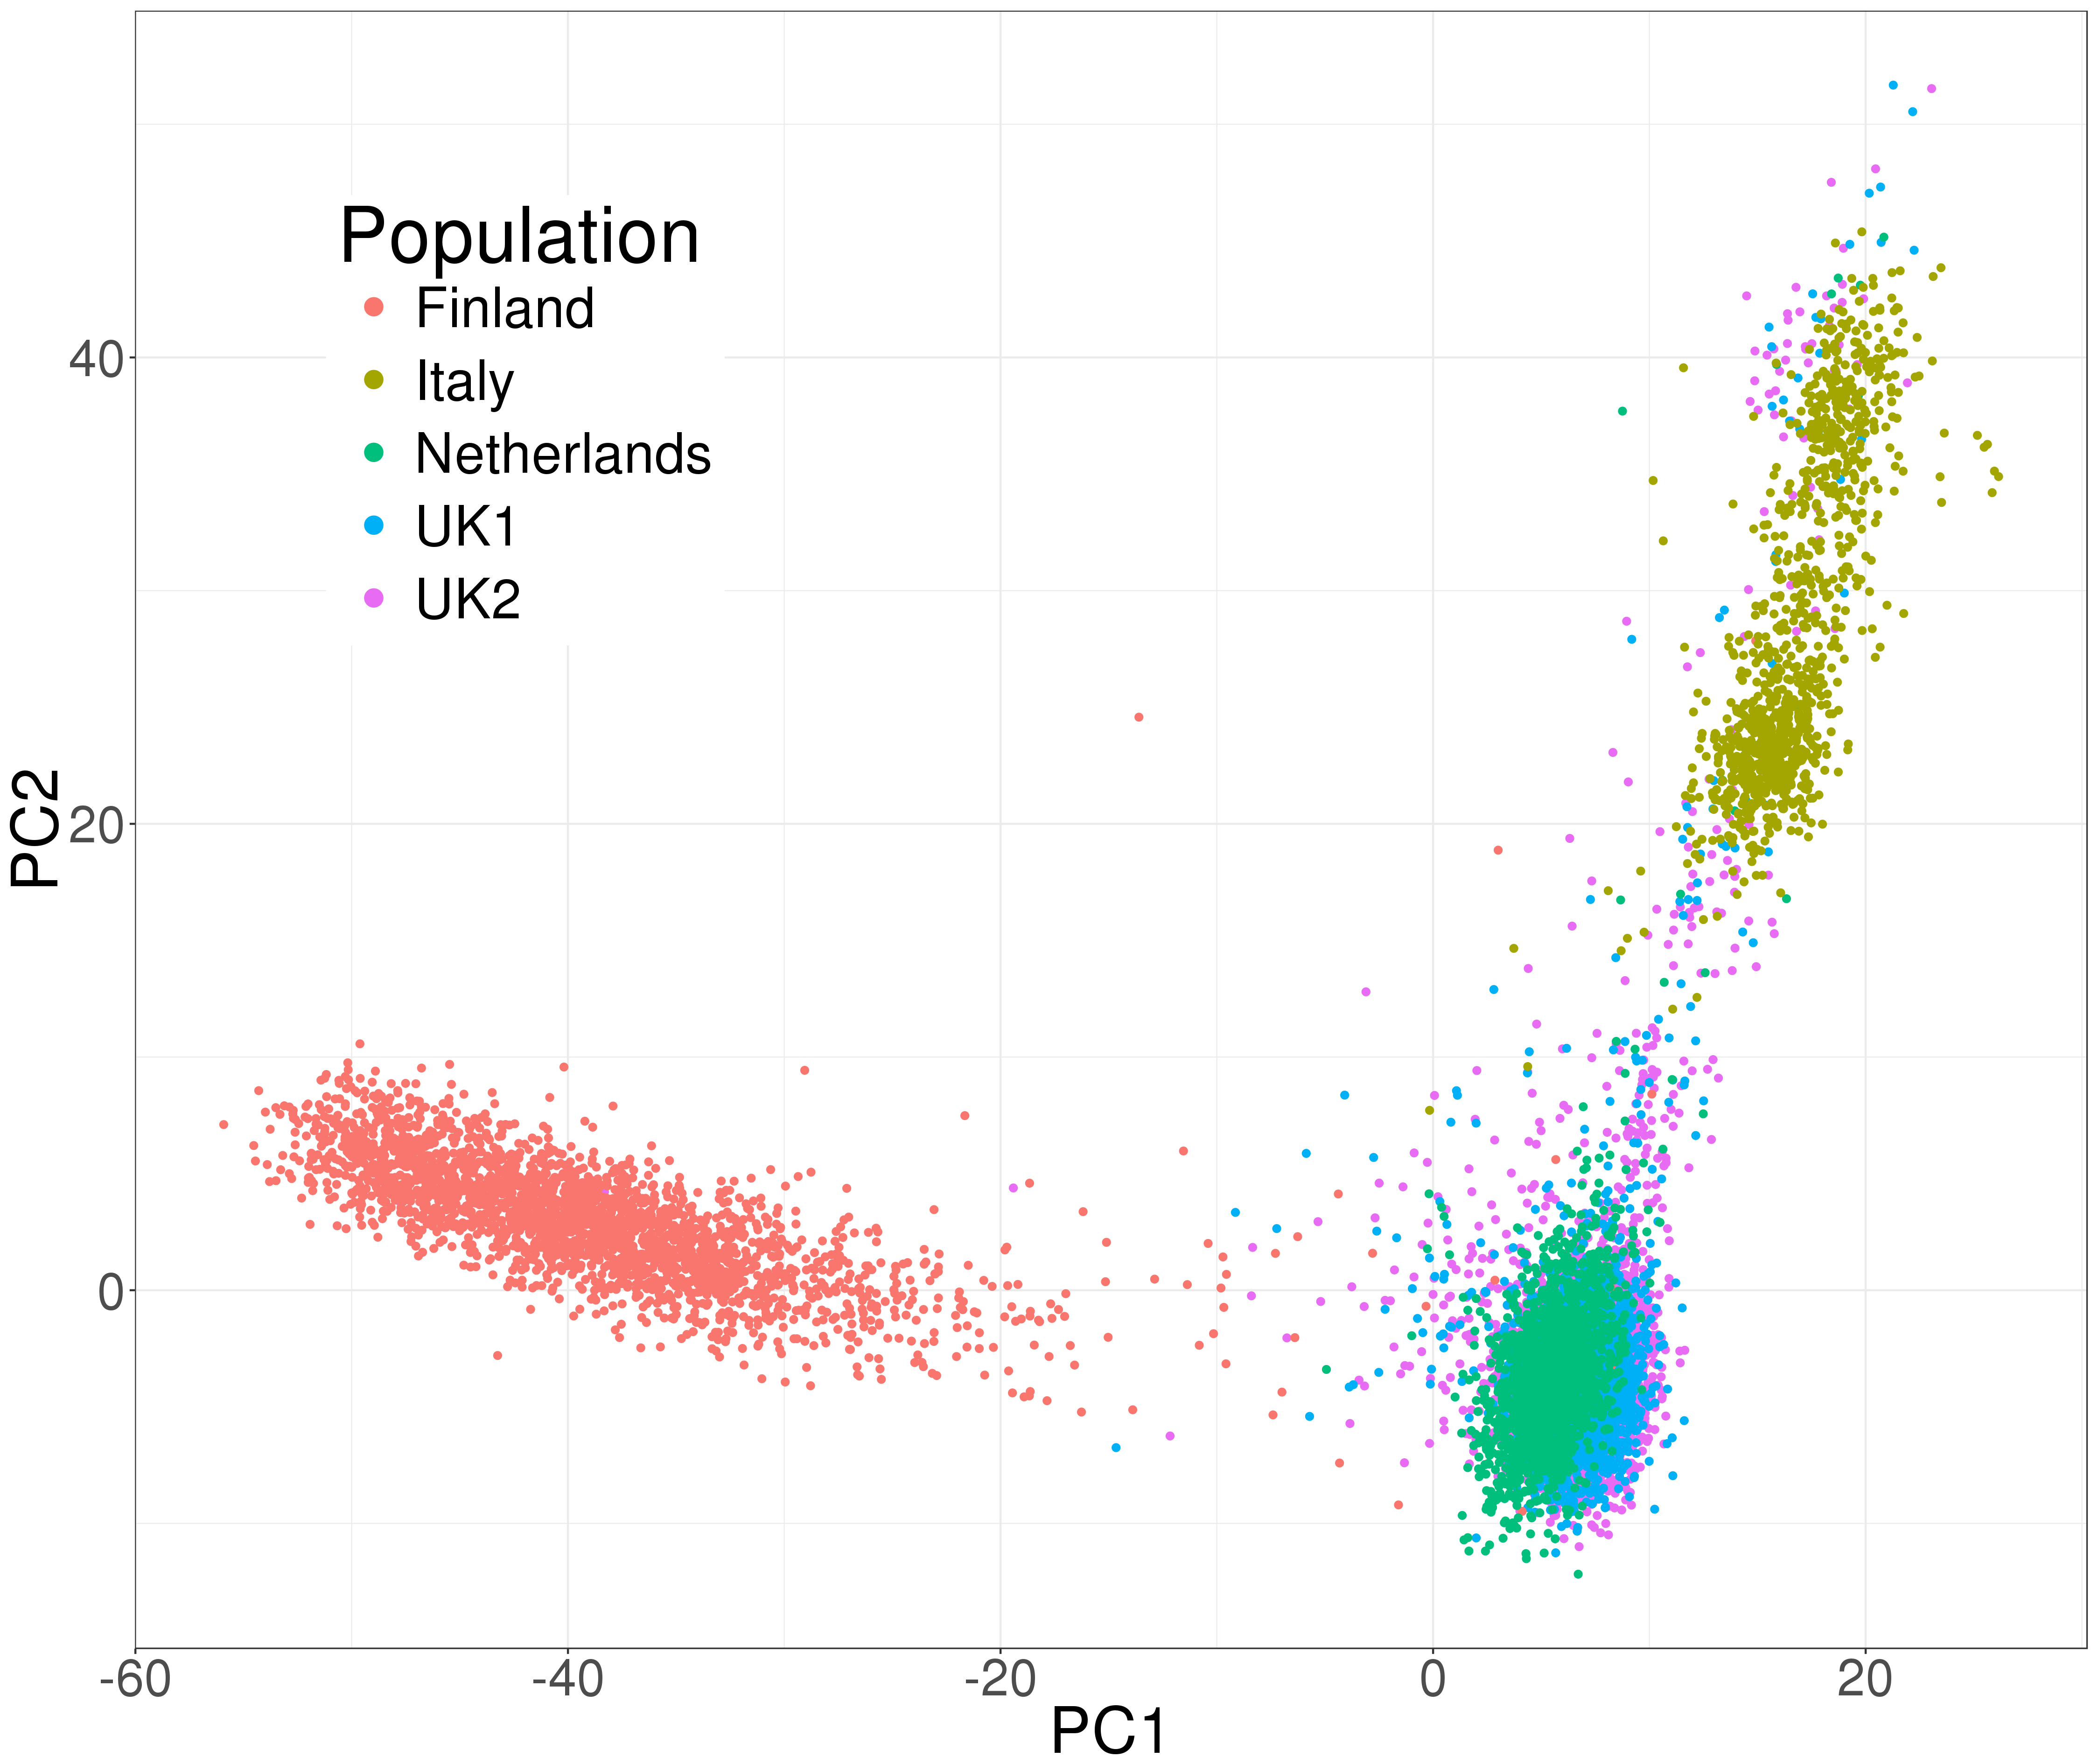
\includegraphics[width=200pt]{celiac-pca}}
\caption{Principal Components of the celiac cohort genotype matrix produced by package bigstatsr.}\label{fig:pca}
\end{figure}

\begin{figure}[!tpb]
\centerline{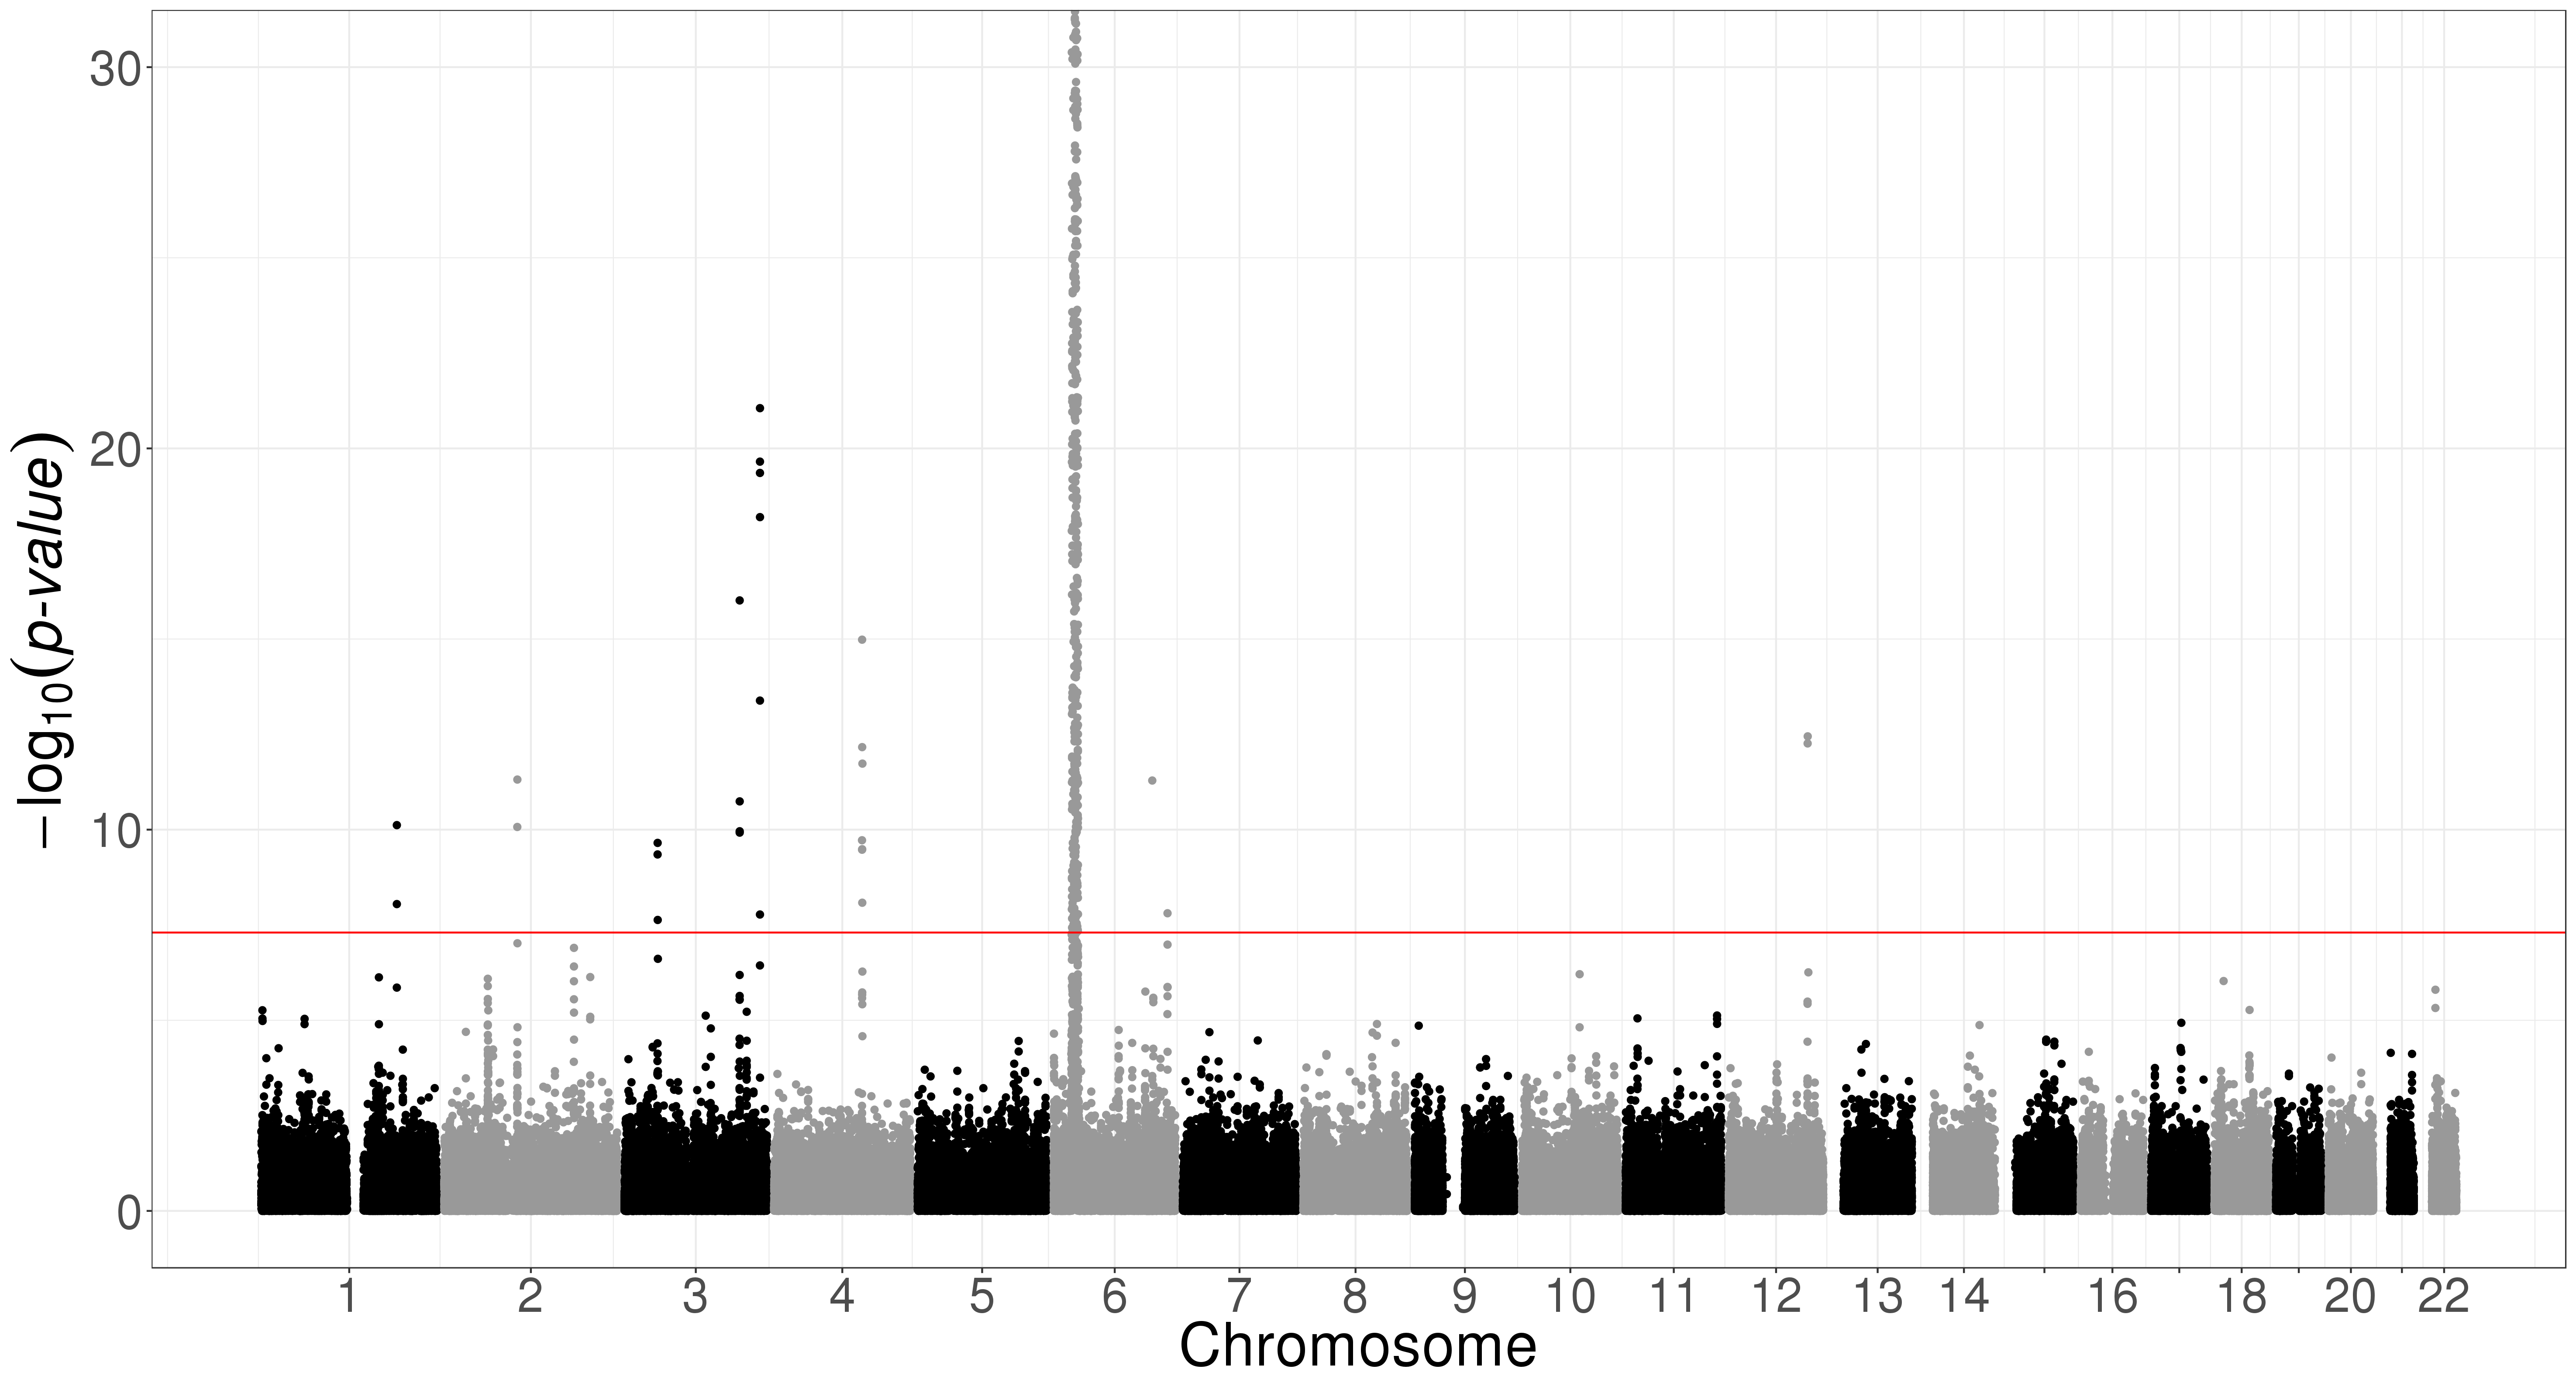
\includegraphics[width=235pt]{celiac-gwas-cut}}
\caption{Manhattan plot of the celiac disease cohort produced by package bigsnpr. Some SNPs in chromosome 6 have p-values smaller than the $10^{-30}$ threshold used for vizualisation purposes.}\label{fig:gwas}
\end{figure}

%The Celiac dataset is relatively small as compared to modern genetic cohorts. 
To illustrate the scalability of the two R packages, we performed a GWAS analysis on 500K individuals and 1M SNPs. The GWAS analysis completed in approximately 11 hours using the aforementioned desktop computer. The GWAS analysis was composed of four main steps. 
First we read from PLINK files in our format "bigSNP" in 1 hour.
Then, we removed SNPs in long-range LD regions and used SNP clumping, leaving 93,083 SNPs in 5.4h. Then, the 10 first PCs were computed on the 500K individuals and these remaining SNPs in 1.8h. Finally, we performed a linear association test on the complete 500K dataset for each of the 1M SNPs, using the 10 first PCs as covariables in 2.9h.

\subsection{Method Comparison}

We first compared the GWAS and PRS computations obtained with the R packages to the ones obtained with PLINK 1.9 and EIGENSOFT 6.1.4.
For most functions, multithreading is not available yet in PLINK, nevertheless, PLINK-specific algorithms that use bitwise parallelism (e.g. pruning) are still faster than the parallel algorithms reimplemented in package bigsnpr (Table~\ref{tab:bench-gwas}). Overall, the computations with our two R packages for an association study and a polygenic risk score are of the same order of magnitude as when using PLINK and EIGENSOFT (Tables~\ref{tab:bench-gwas} and~\ref{tab:bench-prs}). However, the whole analysis pipeline makes use of R calls only; there is no need to write temporary files and functions have parameters which enable subsetting of the genotype matrix without having to copy it. 

\begin{table}[!tpb]
\begin{center}
\begin{adjustbox}{max width=235pt}
\begin{tabular}{|c|c|c|}
\hline
\multirow{2}{*}{Operation} &   \multicolumn{2}{c|}{Execution times (in seconds)} \\
 \cline{2-3}
 & PLINK and FastPCA & bigstatsr and bigsnpr \\
\hline
Reading PLINK files & n/a & 5 / 20 \\
Pruning & 4 / 4 & 14 / 52 \\
Computing 10 PCs & 306 / 315 & 58 / 180 \\
GWAS (binary phenotype) & 339 / 293 & 301 / 861 \\
\hline
Total & 649 / 612 & 378 / 1113 \\
\hline
\end{tabular} 
\end{adjustbox}
\end{center}
\caption{Execution times with bigstatsr and bigsnpr compared to PLINK and FastPCA for making a GWAS for the Celiac dataset. The first execution time is with a desktop computer (6 cores used and 64GB of RAM) and the second one is with a laptop computer (2 cores used and 8GB of RAM).} 
\label{tab:bench-gwas}
\end{table}

\begin{table}[!tpb]
\begin{center}
\begin{adjustbox}{max width=235pt}
\begin{tabular}{|c|c|c|}
\hline
\multirow{2}{*}{Operation} &   \multicolumn{2}{c|}{Execution times (in seconds)} \\
 \cline{2-3}
 & PLINK & bigstatsr and bigsnpr \\
\hline
GWAS (binary phenotype) & 232 / 239 & 178 / 650  \\
Clumping & 49 / 58 & 10 / 35 \\
PRS & 9 / 10 & 2 / 3 \\
\hline
Total & 290 / 307 & 190 / 688 \\
\hline
\end{tabular} 
\end{adjustbox}
\end{center}
\caption{Execution times with bigstatsr and bigsnpr compared to PLINK and FastPCA for making a PRS for a training set of 80\% of the Celiac dataset. The first execution time is with a desktop computer (6 cores used and 64GB of RAM) and the second one is with a laptop computer (2 cores used and 8GB of RAM).}
\label{tab:bench-prs}
\end{table}

On our desktop computer, we compared the computation times of FastPCA, FlashPCA2 to the similar function big\_randomSVD implemented in bigstatsr. For each comparison, we used the 93,083 SNPs which were remaining after pruning and we computed 10 PCs. We used the datasets of growing size simulated from the Celiac dataset. Overall, our function big\_randomSVD showed to be almost twice as fast as FastPCA and FlashPCA2 and 8 times as fast when using parallelism (an option not currently possible with either FastPCA or FlashPCA2) with 6 cores (Figure~\ref{fig:bench-pca}). We also compared results in terms of precision by comparing squared correlation between approximated PCs and ``true'' PCs provided by an exact singular value decomposition obtained with SmartPCA. FastPCA, FlashPCA2 and bigstatsr infer the true first 6 PCs but the squared correlation between true PCs and approximated ones decreases for larger PCs when using FastPCA (Fast mode of EIGENSOFT) whereas it remains larger than 0.999 when using FlashPCA2 or bigstatsr (Figure~\ref{fig:prec-pca}).   

\begin{figure}[!tpb]
\centerline{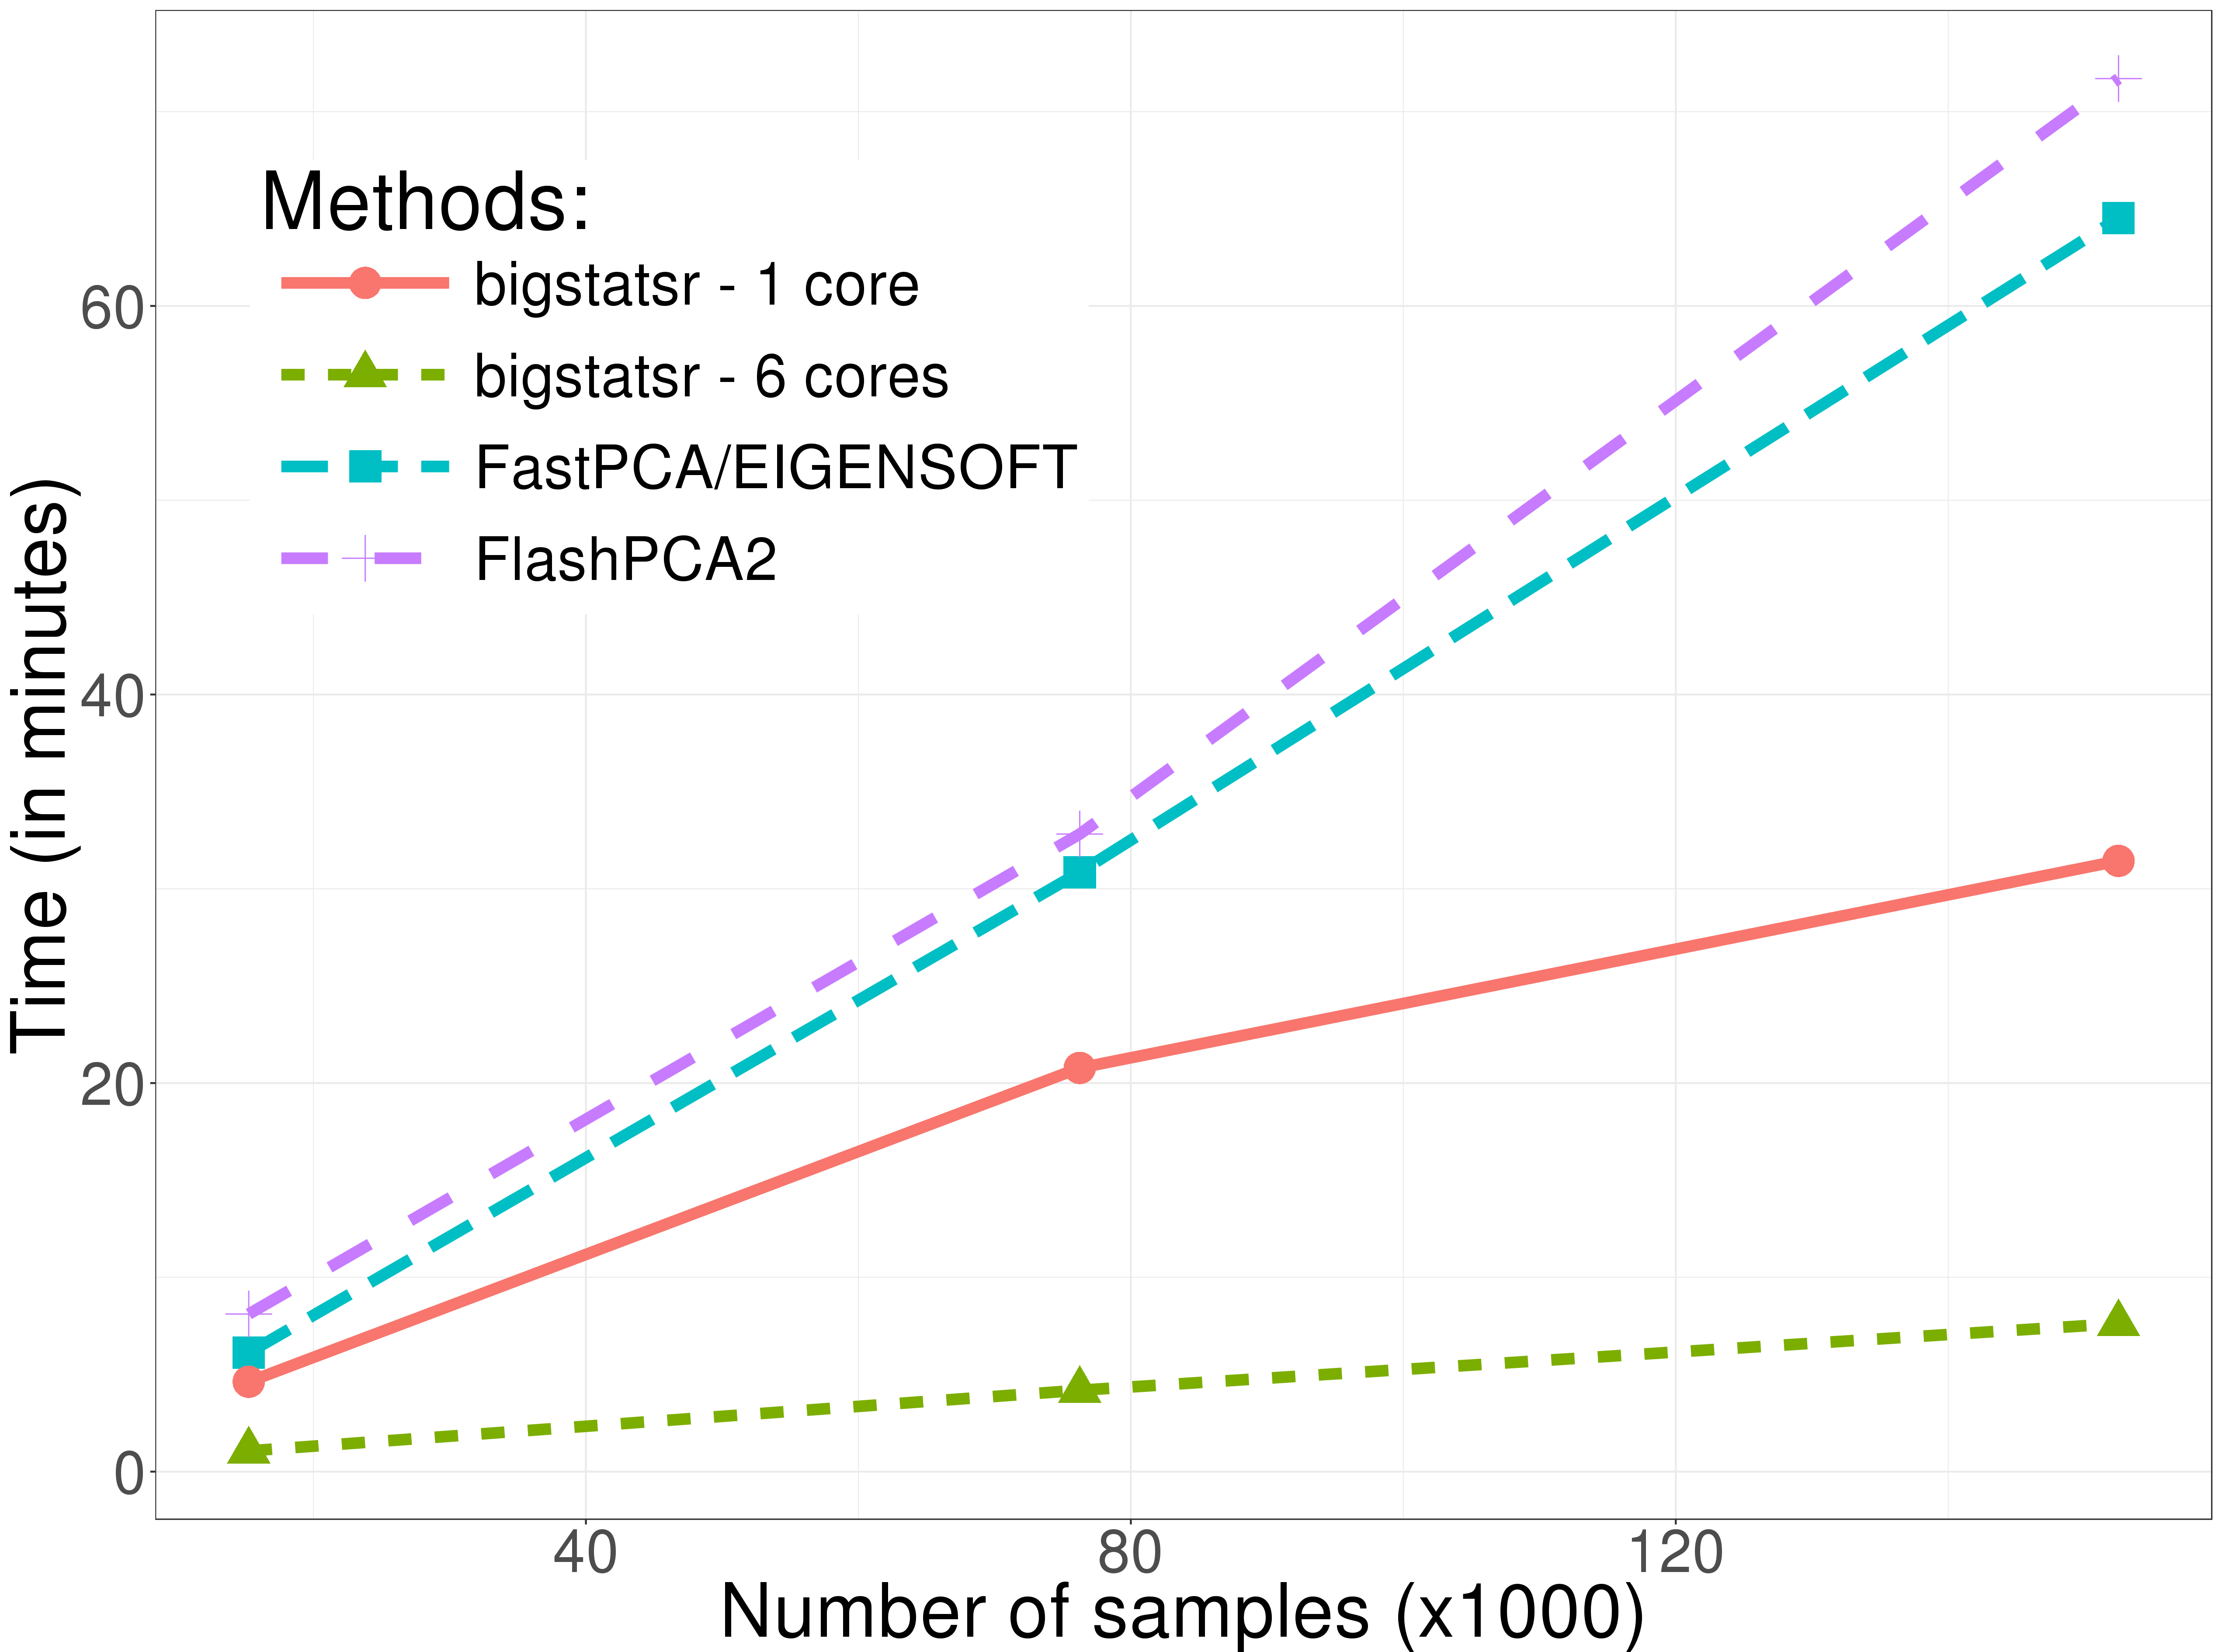
\includegraphics[width=200pt]{benchmark-pca.png}}
\caption{Benchmark comparisons between randomized Partial Singular Value Decomposition available in FlashPCA2, FastPCA (fast mode of SmartPCA/EIGENSOFT) and package bigstatsr. It shows the computation time in minutes as a function of the number of samples. The first 10 principal components have been computed based on the 93,083 SNPs which remained after thinning.}\label{fig:bench-pca}
\end{figure}

\begin{figure}[!tpb]
\centerline{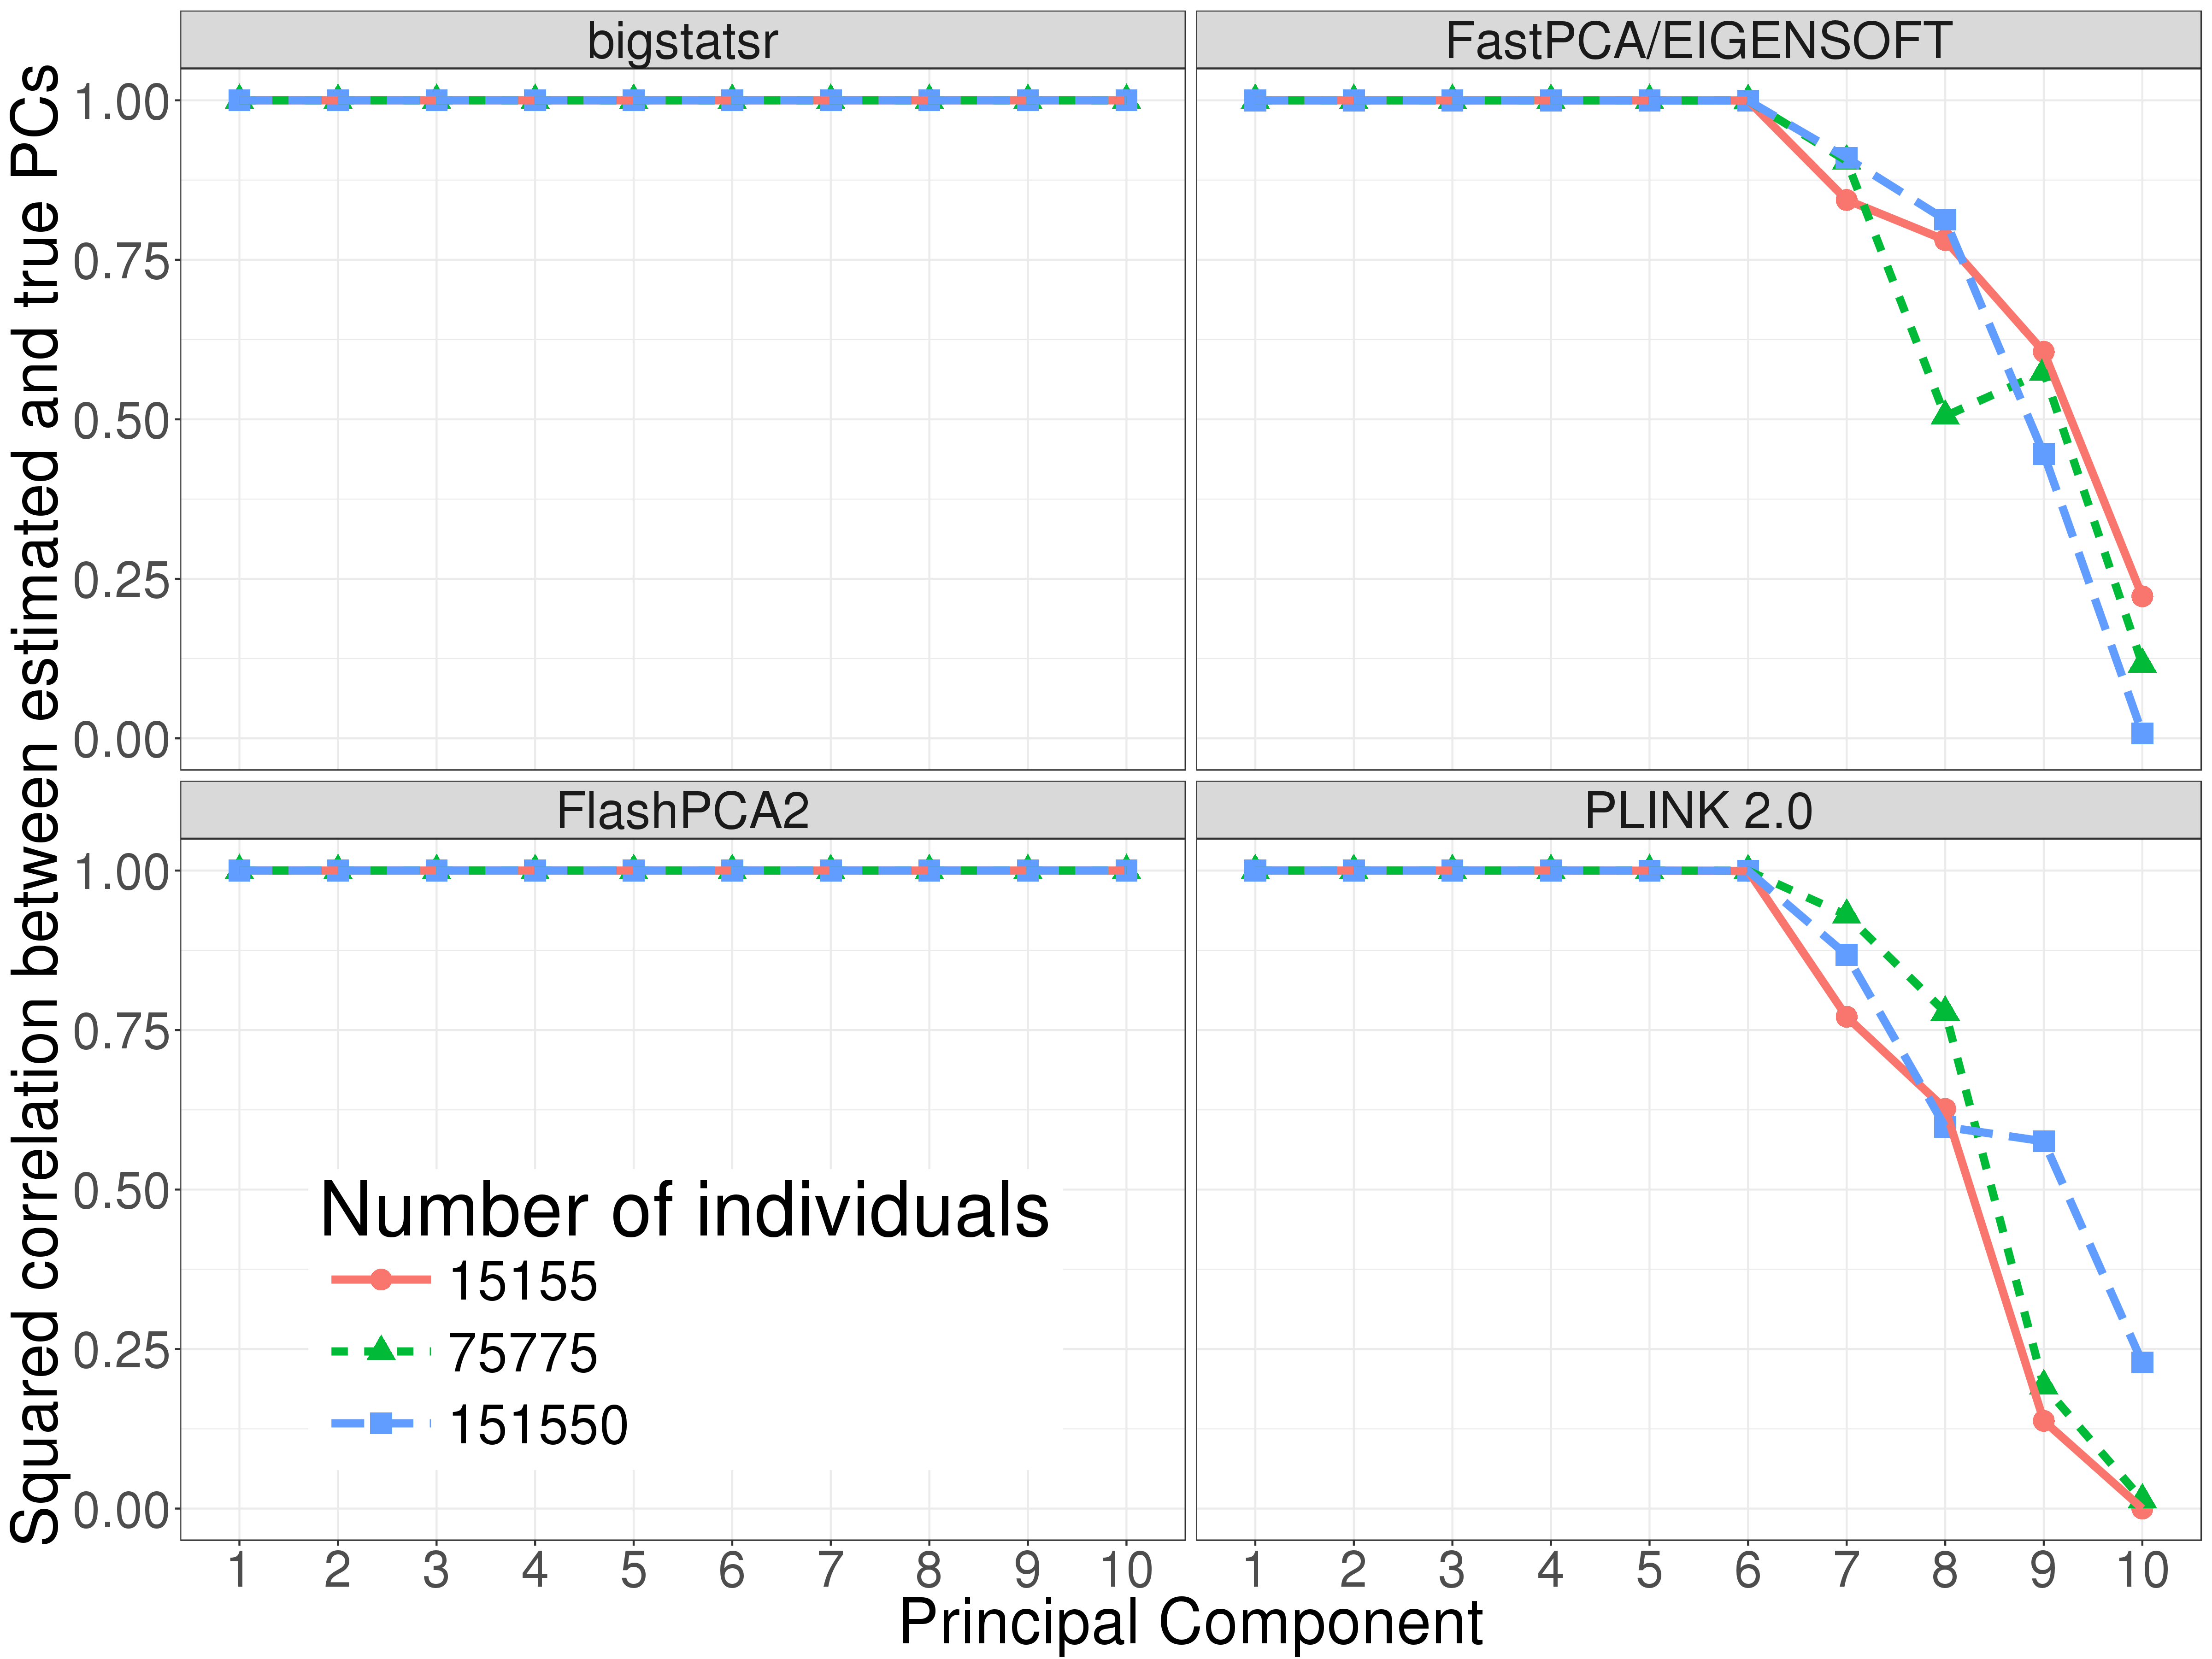
\includegraphics[width=200pt]{precision-pca.png}}
\caption{Precision comparisons between randomized Partial Singular Value Decomposition available in FlashPCA2, FastPCA (fast mode of SmartPCA/EIGENSOFT) and package bigstatsr. It shows the squared correlation between approximated PCs and ``true'' PCs (given by the slow mode of SmartPCA) of the Celiac dataset (whose individuals have been repeated 1, 5 and 10 times).}\label{fig:prec-pca}
\end{figure}

\subsection{Automatic detection of long-range LD regions}

For the detection of long-range LD regions during the computation of PCA, we tested the function snp\_autoSVD on both the Celiac and POPRES datasets. For the POPRES dataset, the algorithm converged in two iterations. The first iterations found 3 long-range LD regions in chromosomes 2, 6 and 8 (Table~\ref{tab:lrldr-popres}). 
We compared the PCs of genotypes obtained after applying snp\_autoSVD with the PCs obtained after removing pre-determined long-range LD regions\footnote{https://goo.gl/8TngVE} and found a mean correlation of 89.6\% between PCs, mainly due to a rotation of PC7 and PC8 (Table~\ref{tab:pc-popres}). For the Celiac dataset, we found 5 long-range LD regions (Table~\ref{tab:lrldr-celiac}) and a mean correlation of 98.6\% between PCs obtained with snp\_autoSVD and the ones obtained by clumping with removing of predetermined long-range LD regions (Table~\ref{tab:pc-celiac}).

For the Celiac dataset, we further compared results of PCA obtained when using snp\_autoSVD and when computing PCA without removing any long range LD region (only clumping at $R^2 > 0.2$). 
When not removing any long range LD region, we show that PC4 and PC5 do not capture population structure and correspond to a long-range LD region in chromosome 8 (Figures~\ref{fig:scores} and~\ref{fig:loadings}). 
When automatically removing some long-range LD regions with snp\_autoSVD, we show that PC4 and PC5 reflect population structure (Figure~\ref{fig:scores}). Moreover, loadings are more equally distributed among SNPs after removal of long-range LD regions (Figure~\ref{fig:loadings}). 
This is confirmed by Gini coefficients (measure of dispersion) of each squared loadings that are significantly smaller when computing SVD with snp\_autoSVD than when no long-range LD region is removed (Figure~\ref{fig:gini}).

\subsection{Imputation of missing values for genotyped SNPs}\label{sec:impute}

For the imputation method based on XGBoost, we compared  the imputation accuracy and computation times with Beagle on the POPRES dataset. The histogram of the minor allele frequencies (MAFs) of this dataset is provided in figure~\ref{fig:maf} and there is no missing value. 
We used a Beta-binomial distribution to simulate the number of missing values by SNP and then randomly introduced missing values according to these numbers, resulting in approximately 3\% of missing values overall (Figure~\ref{fig:NA}). Imputation was compared between function snp\_fastImpute of package bigsnpr and Beagle 4.1 (version of January 21, 2017). Overall, snp\_fastImpute made 4.7\% of imputation errors whereas Beagle made only 3.1\% of errors but it took Beagle 14.6 hours to complete while our method only took 42 minutes (20 times less). 
We also show that the estimation of the number of imputation errors is accurate (Figure~\ref{fig:error-impute}).
For the Celiac dataset in which there was already missing values, in order to further compare computation times, we report that snp\_fastImpute took less than 10 hours to complete for the whole genome whereas Beagle did not finish imputing chromosome 1 in 48 hours. 



\section{Discussion}

We have developed two R packages, bigstatsr and bigsnpr, which enable multiple analyses of large-scale genotype datasets in a single comprehensive framework. Linkage Disequilibrium pruning, Principal Component Analysis, association tests and computations of polygenic risk scores are made available in this software. Implemented algorithms are both fast and memory-efficient, allowing the use of laptops or desktop computers to make genome-wide analyses. 
Technically, bigstatsr and bigsnpr could handle any size of datasets. However, if the OS has to often swap between the file and the memory for accessing the data, this would slow down data analysis. For example, the Principal Component Analysis (PCA) algorithm in bigstatsr is iterative so that the matrix has to be sequentially accessed over a hundred times. If the number of samples times the number of SNPs remaining after pruning is larger than the available memory, this slowdown would happen. For instance, a 32GB computer would be slow when computing PCs on more than 100K samples and 300K SNPs remaining after LD thinning.

The two R packages use a matrix-like format, which makes it easy to develop new functions in order to experiment and develop new ideas. Integration in R makes it possible to take advantage of the vast and diverse R libraries. For example, we developed a fast and accurate imputation algorithm for genotyped SNPs using the widely-used machine learning algorithm XGBoost available in the R package xgboost. Other functions, not presented here, are also available and all the functions available within the package bigstatsr are not specific to SNP arrays, so that they could be used for other omic data or in other fields of research.

We think that the two R packages and the corresponding data format could help researchers to develop new ideas and algorithms to analyze genome-wide data. For example, we wish to use these packages to train much more accurate predictive models than the standard C+T model currently in use when computing Polygenic Risk Scores. As a second example, multiple imputation has been shown to be a very promising method for increasing statistical power of a GWAS \cite[]{Palmer2016}, and it could be implemented with the data format ``FBM.code256'' without having to write multiple files.


\section*{Acknowledgements}

Authors acknowledge Grenoble Alpes Data Institute, supported by the French National Research Agency under the ``Investissements d'avenir'' program (ANR-15-IDEX-02) and the LabEx PERSYVAL-Lab (ANR-11-LABX-0025-01).

\vspace*{-12pt}

\bibliographystyle{natbib}
\bibliography{document}

\end{document}
